\chapter{Integration and Control of Subsystems}

This chapter outlines the integration process between MBDyn and \textit{Simulink}, relevant concepts in \textit{Simulink} and control theory, and the architecture of the \textit{Simulink} control system. Following construction, the foundational control system is evaluated, and the typical control responses are examined.

\section{Concepts of Reference Frames and Rotation}

In aerospace engineering and navigation, a comprehensive grasp of reference frames and rotational principles is indispensable for accurately characterizing object and vehicle movements. These concepts underpin navigation, control, and simulation across various domains.

\subsection[Global Navigation Frame N]{Global Navigation Frame $\overrightarrow{\mathcal{N}}$}

The global navigation frame establishes a universal reference for delineating an object's motion relative to the Earth's surface. Typically, it is defined using Earth-centered coordinates like latitude, longitude, and altitude. Notable instances encompass the Earth-Centered, Earth-Fixed (ECEF) frame and the Geodetic frame. This frame furnishes a steadfast benchmark for navigation systems, enabling precise object localization and tracking across expansive geographic regions.

\subsection[Local Vertical Frame (NED)]{Local Vertical Frame (NED) $\mathcal{N}$}

The local vertical frame, also referred to as the North-East-Down (NED) frame, serves as a localized reference frame extensively employed in aircraft navigation and control. Centered at the vehicle's position, it aligns its $x$-axis with north, $y$-axis with east, and $z$-axis with the downward direction toward the Earth's center. Facilitating navigation and control algorithms, the NED frame provides an intuitive reference for elucidating the vehicle's motion in relation to its environment.

\subsection[Vehicle Body Frame]{Vehicle Body Frame $\mathcal{B}$}

The vehicle body frame serves as a reference frame fixed to the vehicle's structure. Aligned with the vehicle's movements and rotations, it provides a convenient framework for describing its motion and dynamics. Typically, the $x$-, $y$-, and $z$-axes of the body frame correspond to the vehicle's longitudinal, lateral, and vertical axes, respectively. Crucial for analyzing and managing the vehicle's motion, the body frame offers a reference relative to which forces and torques can be computed and applied.

\subsection[Wind Frame]{Wind Frame $\mathcal{W}$}

The wind frame constitutes a reference frame moving with the air mass surrounding the vehicle. It proves particularly valuable for scrutinizing aerodynamic forces and moments acting on an aircraft. In the wind frame, the $x$-axis aligns with the direction of the relative wind, the $y$-axis is perpendicular to the relative wind in the horizontal plane, and the $z$-axis points upward. Facilitating precise analysis of the vehicle's aerodynamic performance, the wind frame accommodates considerations of wind effects on its motion.

\begin{figure}
    \centering
    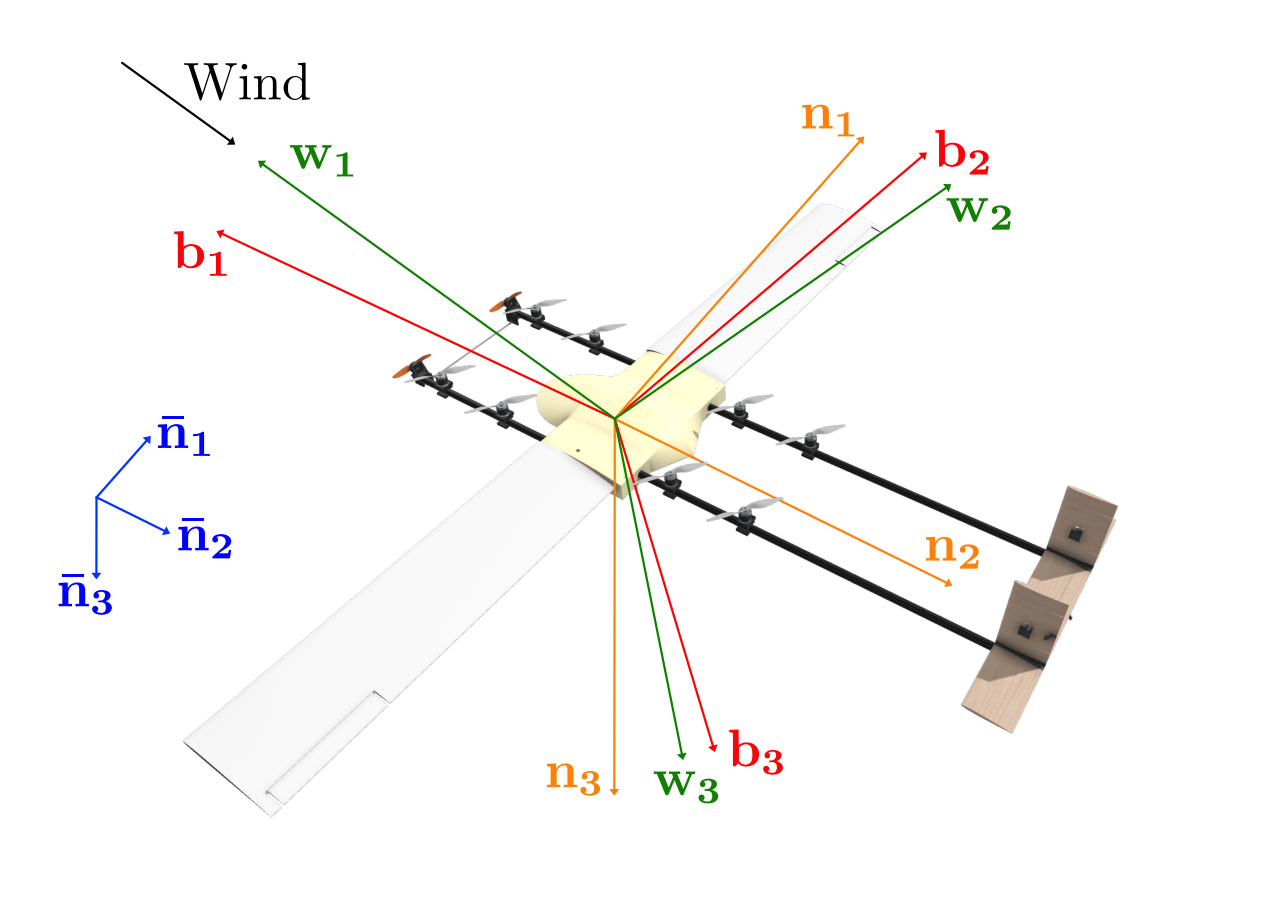
\includegraphics[width=0.8\linewidth]{Images/reference_frame.png}
    \caption{Schematic representation of reference frames.}
    \label{fig:reference_frames}
\end{figure}

\subsection{Rotation Formalism}

Rotation formalism is used to represent the orientation of an object or coordinate frame relative to another frame. Common representations include Euler angles, time derivatives of Euler angles, and quaternions.

\subsubsection{Euler Angles}
The Euler angles (called roll \(\phi\), pitch \(\theta\) and yaw \(\psi\)) are three independent angular quantities able to describe the 3D orientation of an object, using two sets of reference frames: an inertial Earth-fixed one and a body one, rigidly attached to the object. The Euler angles define the transformation of the components of a generic vector between two sets of axes. A vector \(\mathbf{v}_A\) in the initial reference frame \(A\) can be rotated into the reference frame \(B\) obtaining \(\mathbf{v}_B\), with the rotation matrix \(\mathbf{R}_{B}^{A}\):
\begin{equation}
    \mathbf{v}_B = \mathbf{R}_{A}^{B} \mathbf{v}_A. \label{eq:rotation_matrix}
\end{equation}
Any arbitrary attitude is obtained by an ordered sequence of three consecutive rotations around each axis of an orthogonal frame; the rotation around the \(x\) axis can be described with matrix \(R_x(\phi)\):
\begin{equation}
    R_X(\phi) = \begin{bmatrix} 
        1 & 0 & 0 \\ 
        0 & \cos \phi & \sin \phi \\ 
        0 & -\sin \phi & \cos \phi 
    \end{bmatrix}, \label{eq:rotation_x}
\end{equation}
while, in similar fashion the rotation around \(y\) and \(z\) are described respectively with rotation matrices \(R_y(\theta)\), \(R_z(\psi)\):
\begin{align}
    R_Y(\theta) &= \begin{bmatrix} 
        \cos \theta & 0 & -\sin \theta \\ 
        0 & 1 & 0 \\ 
        \sin \theta & 0 & \cos \theta 
    \end{bmatrix}, \label{eq:rotation_y} \\
    R_Z(\psi) &= \begin{bmatrix} 
        \cos \psi & \sin \psi & 0 \\ 
        -\sin \psi & \cos \psi & 0 \\ 
        0 & 0 & 1 
    \end{bmatrix}. \label{eq:rotation_z}
\end{align}
In aircraft dynamics, the generic attitude of the vehicle is obtained by the so-called rotation sequence 321: the attitude of the body axes \(B\) (always aligned with the aircraft) with respect to a non-rotating NED \(N\) reference frame, is obtained by a first rotation about the \(z\) axis of an angle \(\psi\), then a rotation about the \(y\) axis of an angle \(\theta\), and finally a rotation about the \(x\) axes of an angle \(\phi\). The final rotation matrix from \(N\) to \(B\) is obtained by the ordered multiplication of the previous rotation matrices (equations \eqref{eq:rotation_x}, \eqref{eq:rotation_y}, and \eqref{eq:rotation_z}); it is called Euler rotation matrix and has the following expression:
\begin{equation}
    \mathbf{T}_{N}^{B}(\phi, \theta, \psi) = \begin{bmatrix} 
        C_{\theta}C_{\psi} & C_{\theta}S_{\psi} & -S_{\theta} \\ 
        S_{\phi}S_{\theta}C_{\psi} - C_{\phi}S_{\psi} & S_{\phi}S_{\theta}S_{\psi} + C_{\phi}C_{\psi} & S_{\phi}C_{\theta} \\ 
        C_{\phi}S_{\theta}C_{\psi} + S_{\phi}S_{\psi} & C_{\phi}S_{\theta}S_{\psi} - S_{\phi}C_{\psi} & C_{\phi}C_{\theta} 
    \end{bmatrix}, \label{eq:euler_rotation_matrix}
\end{equation}
where \(C_{\alpha} = \cos(\alpha)\) and \(S_{\alpha} = \sin(\alpha)\) for the sake of brevity.
The roll angle \(\phi\), the pitch angle \(\theta\), and the yaw angle \(\psi\) are grouped in the vector \(\boldsymbol{\alpha}_e\), which uniquely describes the aircraft’s attitude in space with respect to the NED reference frame \(N\):
\begin{equation}
    \boldsymbol{\alpha}_e = \begin{bmatrix} 
        \phi \\ 
        \theta \\ 
        \psi 
    \end{bmatrix}. \label{eq:euler_angles_vector}
\end{equation}

\subsubsection{Time derivatives of Euler angles}
The attitude of an aircraft changes with time when the aircraft maneuvers. The Euler angle rates are a function of the Euler angles and body-axis angular rates. The components of the angular velocity measured in the body frame \(\omega_B\) are the roll rate \(p\), pitch rate \(q\), and yaw rate \(r\):
\begin{equation}
    \boldsymbol{\omega}_B = \begin{bmatrix} 
        p \\ 
        q \\ 
        r 
    \end{bmatrix}. \label{eq:angular_velocity}
\end{equation}
The rate of change of Euler angles is related to \(\omega_B\) by the following equation:
\begin{equation}
    \dot{\boldsymbol{\alpha}}_e = E^{-1} \boldsymbol{\omega}_B, \label{eq:euler_angle_rate}
\end{equation}
with \(E^{-1}\) being the inverse of matrix \(E\), whose expressions are given by:
\begin{align}
    E(\phi, \theta) &= \begin{bmatrix} 
        1 & 0 & -\sin \theta \\ 
        0 & \cos \phi & \sin \phi \cos \theta \\ 
        0 & -\sin \phi & \cos \phi \cos \theta 
    \end{bmatrix}, \label{eq:matrix_E} \\
    E^{-1}(\phi, \theta) &= \begin{bmatrix} 
        1 & \sin \phi \tan \theta & \cos \phi \tan \theta \\ 
        0 & \cos \phi & -\sin \phi \\ 
        0 & \frac{\sin \phi}{\cos \theta} & \frac{\cos \phi}{\cos \theta} 
    \end{bmatrix}. \label{eq:matrix_E_inverse}
\end{align}
It can be seen that matrix \(E\) is singular for pitch angles of \(\pm 90^\circ\); this singularity is called gimbal lock and can be avoided using quaternions.
\subsubsection{Quaternions}
A quaternion \( q \) is a parametrization of the four-dimensional unit sphere that can be used to represent the orientation of a rigid body or a coordinate frame in three-dimensional space:
\begin{equation}
    q = \begin{bmatrix} 
        q_0 \\ 
        q_1 \\ 
        q_2 \\ 
        q_3 
    \end{bmatrix}, \quad ||q|| = 1.    
\end{equation}
The quaternion elements generate the following rotation matrix (analogous to the one expressed in Equation \eqref{eq:euler_rotation_matrix} in terms of Euler angles):
\begin{equation}
\mathbf{T}_{N}^{B} = \begin{bmatrix} 
    q_0^2 + q_1^2 - q_2^2 - q_3^2 & 2(q_1q_2 + q_0q_3) & 2(q_1q_3 - q_0q_2) \\ 
    2(q_1q_2 - q_0q_3) & q_0^2 - q_1^2 + q_2^2 - q_3^2 & 2(q_2q_3 + q_0q_1) \\ 
    2(q_1q_3 + q_0q_2) & 2(q_2q_3 - q_0q_1) & q_0^2 - q_1^2 - q_2^2 + q_3^2 
\end{bmatrix}.
\end{equation}
The Euler angles \(\phi\), \(\theta\), and \(\psi\) can be obtained from the elements of the quaternion expressing the aircraft’s orientation with respect to a non-rotating frame through
\begin{align}
    \phi &= \tan^{-1} \left( \frac{2q_3q_4 - 2q_1q_2}{2q_1^2 - 1 + 2q_4^2} \right), \label{eq:euler_angles_phi} \\
    \theta &= -\sin^{-1}(2q_2q_4 + 2q_1q_3), \label{eq:euler_angles_theta} \\
    \psi &= \tan^{-1} \left( \frac{2q_2q_3 - 2q_1q_4}{2q_1^2 - 1 + 2q_2^2} \right). \label{eq:euler_angles_psi}
\end{align}
The quaternion conjugate, denoted by \( (\cdot)^* \), can be used to swap the frames described by an orientation. To follow the previous example, the orientation of frame \( B \) with respect to frame \( A \) can be described by the quaternion \( q_{AB} \), and its conjugate \( q_{AB}^* \) describes the orientation of frame \( A \) relative to frame \( B \) (\( q_{BA} \)), like in the following equation:
\begin{equation}
q_{AB}^* = q_{BA} = \begin{bmatrix} 
    q_0 \\ 
    -q_1 \\ 
    -q_2 \\ 
    -q_3 
\end{bmatrix}.
\end{equation}

The quaternion product, denoted as \( (\otimes) \), is used to describe successive rotations and can be determined using the Hamilton rule, as expressed by Equation \eqref{eq:qac}. The quaternion product is not commutative.
\begin{equation}
q_{AC} = q_{BC} \otimes q_{AB} = \begin{bmatrix} 
    a_0 \\ 
    a_1 \\ 
    a_2 \\ 
    a_3 
\end{bmatrix} \otimes \begin{bmatrix} 
    b_0 \\ 
    b_1 \\ 
    b_2 \\ 
    b_3 
\end{bmatrix} = \begin{bmatrix} 
    a_1b_1 - a_2b_2 - a_3b_3 - a_4b_4 \\ 
    a_1b_2 + a_2b_1 + a_3b_4 - a_4b_3 \\ 
    a_1b_3 - a_2b_4 + a_3b_1 + a_4b_2 \\ 
    a_1b_4 + a_2b_3 - a_3b_2 + a_4b_1 
\end{bmatrix}.  \label{eq:qac}
\end{equation}
A three-dimensional vector can be rotated by a quaternion using Equation \eqref{eq:vb_qbc} by appending a zero as the first element of the vector to make it dimensionally consistent with quaternions:
\begin{equation}
    \mathbf{v}_B = q_{AB} \otimes \mathbf{v}_A \otimes q_{AB}^*,    \label{eq:vb_qbc}
\end{equation}
where \( \mathbf{v}_A \) and \( \mathbf{v}_B \) are the same vector described in frame A and frame B, respectively.

Finally, the quaternion derivative describing the rate of change of orientation of the Earth frame relative to the body frame can be calculated by the equation:
\begin{equation}
\dot{q}_{BE} = \frac{1}{2} q_{BE} \otimes \boldsymbol{\omega}, \quad \text{where} \quad \boldsymbol{\omega} = \begin{bmatrix} 0 \\ \omega_B \end{bmatrix}, \label{eq:q_BE}
\end{equation}
Resolving Equation \eqref{eq:q_BE} leads to
\begin{equation}
    \begin{bmatrix} 
        \dot{q}_1 \\ 
        \dot{q}_2 \\ 
        \dot{q}_3 \\ 
        \dot{q}_4 
    \end{bmatrix} = \frac{1}{2} \begin{bmatrix} 
        0 & -p & -q & -r \\ 
        p & 0 & r & -q \\ 
        q & -r & 0 & p \\ 
        r & q & -p & 0 
    \end{bmatrix} \begin{bmatrix} 
        q_1 \\ 
        q_2 \\ 
        q_3 \\ 
        q_4 
    \end{bmatrix}.    
\end{equation}

\section{Integration with Airframe in MBDyn}

MBDyn offers a variety of modules for interfacing with different software platforms, such as \textit{Simulink}, enabling real-time data exchange with MBDyn to maintain consistent configurations in the model. In the \textit{Simulink} model, the time step is set to \(10^{-3}\) seconds.

\begin{sidewaysfigure}
    \centering
    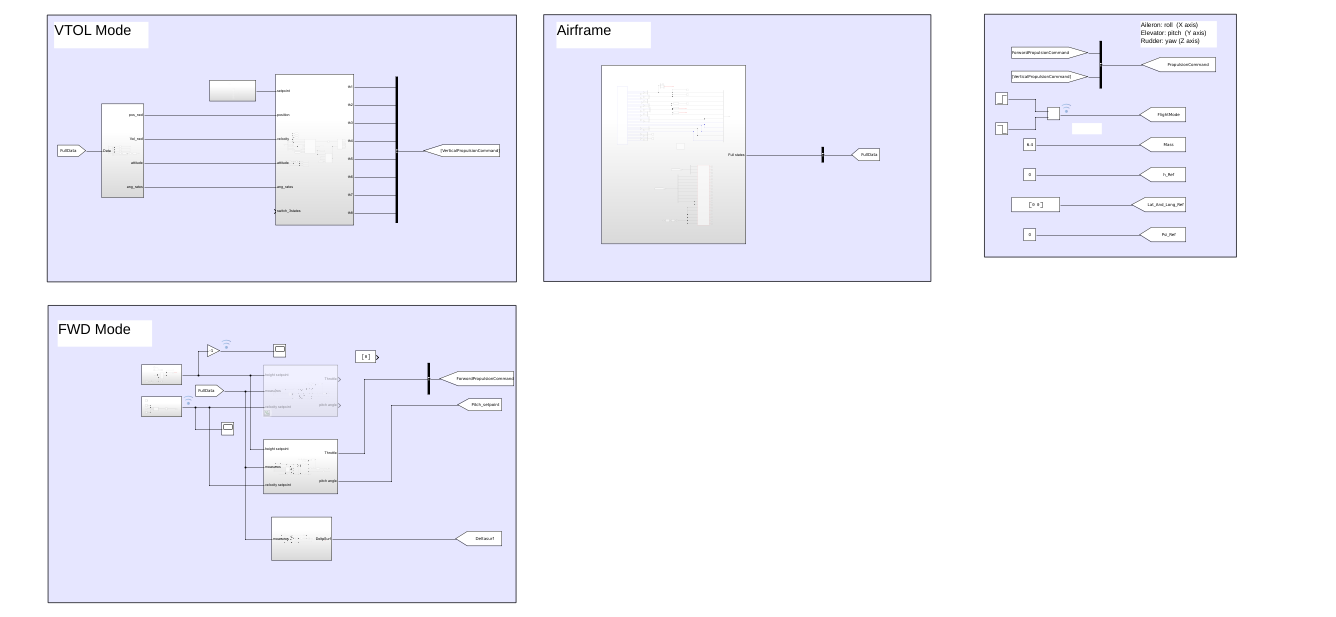
\includegraphics[width=1\linewidth]{Images/SImulink_overview.png}
    \label{fig:Simulink_overview}
    \caption{Overview of the \textit{Simulink} Control System}
\end{sidewaysfigure}

\section{\textit{Simulink} Control System}

The \textit{Simulink} model remains consistent with the description provided in \cite{battaini2022}, featuring both multi-copter and fixed-wing modes within the control system. Inputs and outputs have been adjusted for communication with the MBDyn model.

The \textit{Simulink} module sends 13 control command signals to the MBDyn system, comprising 1-3 ports for movable surfaces (aileron, elevator, rudder), 4-11 ports for throttle command for vertical motors, and 12-13 ports for throttle command for horizontal motors. Conversely, the \textit{Simulink} module receives status information from the MBDyn module, encompassing a total of 35 received signals as outlined in Table \ref{tab:output element}. The integrated MBDyn send and receive module in \textit{Simulink} is depicted in Figure \ref{fig:Simulink_Block_connect_with_MBDyn}.

Since all data output from the MBDyn simulation is in either the global frame, body frame, or wind frame, within the \textit{Simulink} control system, all data is utilized in the global navigation frame, vehicle body frame, or wind frame. Consequently, data is rotated to the corresponding frame using a gain block with a value of -1 before being utilized in the control system.

\begin{sidewaysfigure}
  \centering
  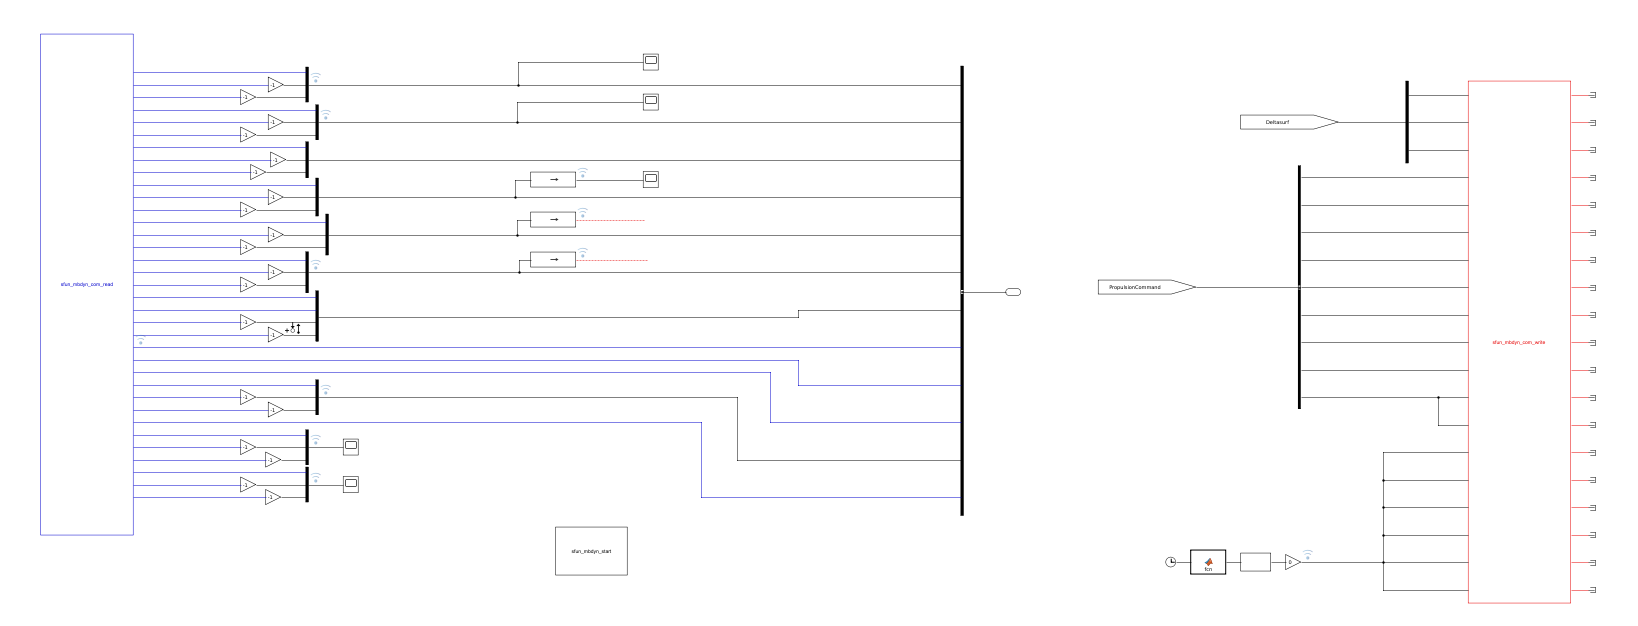
\includegraphics[width=1\linewidth]{Images/airframe.png}
  \caption{Integration of Simulink Block with MBDyn}
  \label{fig:Simulink_Block_connect_with_MBDyn}
\end{sidewaysfigure}

\subsection{Multi-Copter Mode}

The multicopter controller architecture described in \cite{battaini2022} consists of standard cascaded loops with PID controllers derived from \cite{px4controller}. Four loops are present: on the body angular rates, on the attitude angles, on the inertial velocity, and on the inertial position. The structure of the controller \cite{Px4AutopilotWebsite} is depicted in Figure \ref{fig:Multicopter_controller}: a proportional controller \(P\) is used for position and attitude control, while a proportional, integral, and derivative (PID) controller is used for rates and velocity control. The final outputs of the controller are the vertical body force \(T\) and body moments \(L\), \(M\), \(N\), which are converted into motor angular velocities \(\Omega\) with the pseudo-inverse of the mixer matrix \(\chi\), and then into throttle commands \(th\) with the relation \cite{Px4DiscussionForum}:

\begin{equation}
    th = a \Omega^2 + b \Omega, \label{eq:throttle}
\end{equation}

as found in Chapter \ref{ch:chapter1}.

\begin{figure}[h]
    \centering
    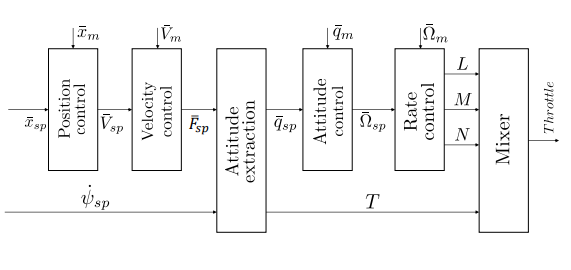
\includegraphics[width=0.9\linewidth]{Images/Multicopter controller.png}
    \caption{Multicopter controller.}
    \label{fig:Multicopter_controller}
\end{figure}

The Simulink implementation of the controller is depicted in Figure \ref{fig:VTOL_controller}. Three main subsystems are visible:

\begin{itemize}
    \item Position controller block, which calculates the body force \(T\) and the desired attitude from position/velocity setpoint;
    \item Attitude controller block, which calculates body moments \(L\), \(M\), \(N\) from attitude setpoint;
    \item Mixer block, which transforms force and moments into throttle commands.
\end{itemize}

The details of the position controller block are shown in Figure \ref{fig:position_controller}: including the position control, velocity control, and setpoint attitude extraction subsystems. Saturation limits are introduced to account for propulsion limits. An integral reset flag is added to avoid continuous error integration by the controller when the multi-rotor is not flying: if the thrust command value is below 20\%, the integration is stopped. There is a feed-forward term on the acceleration setpoint, and the constant force contribution of the weight is considered. The in-plane thrust suppression block manages the force contribution when the drone is on the ground: in this condition, the force is maintained at an idle value until the thrust command reaches 20\%. Additionally, during ALTITUDE MODE, the in-plane thrust suppression block cancels the horizontal component of the force.

The attitude controller block is depicted in Figure \ref{fig:attitude_controller}, composed of attitude and rate control with saturation limits and integral reset.

The attitude controller is based on \cite{brescianini2013nonlinear} and makes use of quaternions \([q_x, q_y, q_z, q_w]\). The drone is an under-actuated mechanical system since it has a lower number of control inputs than the number of degrees of freedom to be controlled: the force generated is oriented in the body vertical direction, so it can only accelerate along this axis. Therefore, the force setpoint \(\bar{F}_{\text{sp}}\) calculated by the velocity controller is transformed into a target orientation \(\bar{q}_{\text{sp}}\), such that the corresponding z-axis is aligned with the desired force.

\begin{sidewaysfigure}
  \centering
      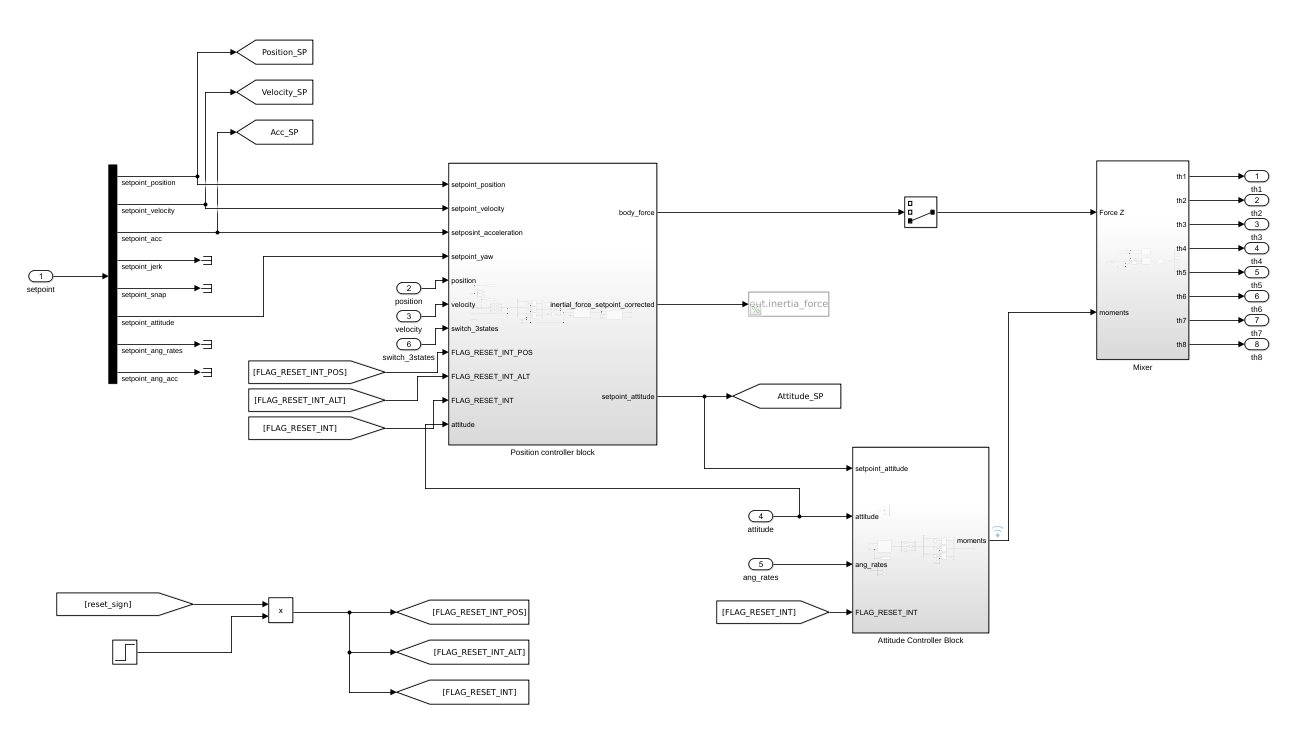
\includegraphics[width=1\linewidth]{Images/VTOL_controller.png}
      \caption{VTOL controller block}
      \label{fig:VTOL_controller}
\end{sidewaysfigure}

\begin{sidewaysfigure}
  \centering
      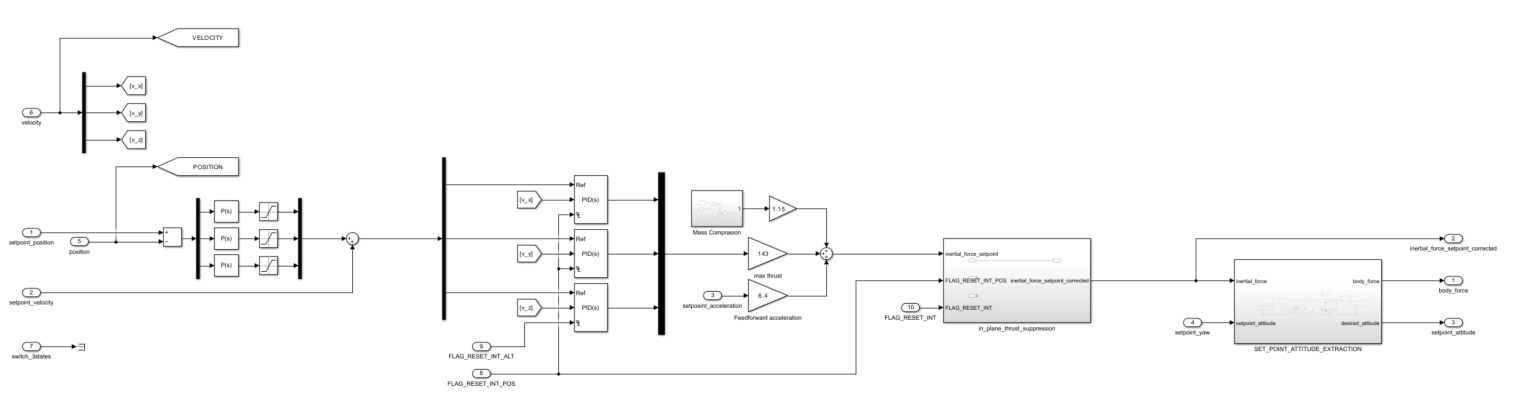
\includegraphics[width=1\linewidth]{Images/position_controller.png}
      \caption{Position controller block}
      \label{fig:position_controller}
\end{sidewaysfigure}

\begin{sidewaysfigure}
  \centering
      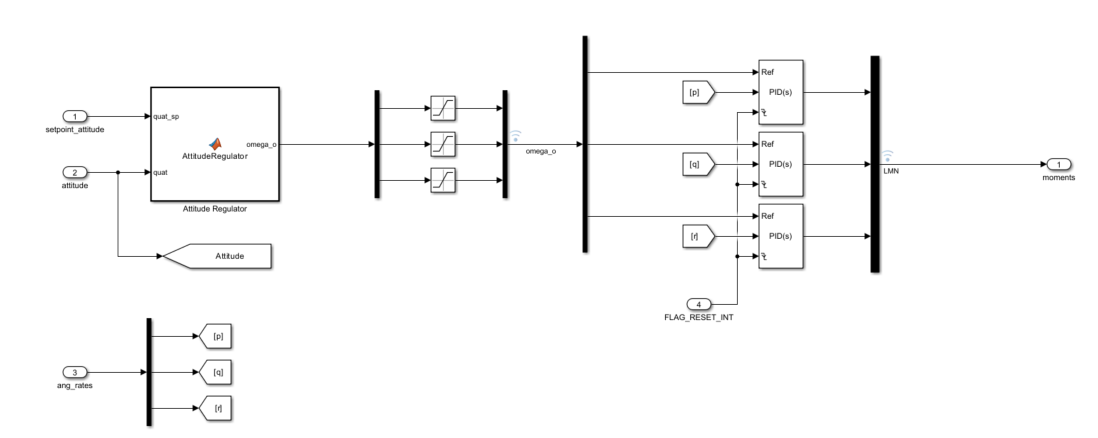
\includegraphics[width=1\linewidth]{Images/attitude_controller.png}
      \caption{Attitude controller block}
      \label{fig:attitude_controller}
\end{sidewaysfigure}

\begin{sidewaysfigure}
  \centering
      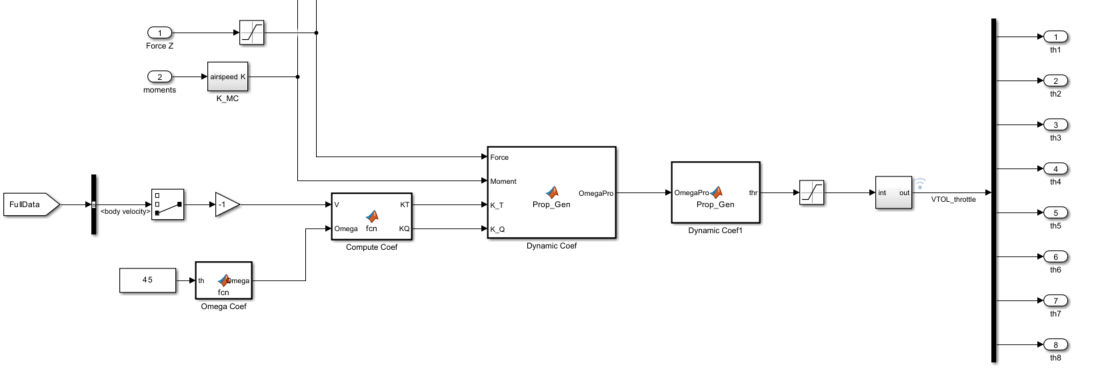
\includegraphics[width=1\linewidth]{Images/mixer_control.png}
      \caption{Mixer controller block}
      \label{fig:mixer_control}
\end{sidewaysfigure}

\subsubsection{Notch Filter}

Significant effort was dedicated to selecting proportional gains to strike a balance between tracking performance and minimizing vibrations. However, even after the tuning campaign, noticeable vibrations persisted. Visual analysis suggested that these vibrations originated in the wings and propagated throughout the entire vehicle. To confirm this hypothesis, a flight was conducted without wings, resulting in the absence of vibrations, thus validating their origin. To address this issue, a notch filter was introduced to exclude the contribution of wing vibrations to the controller action. The notch filter is defined as:
\begin{equation}
    N(s) = \frac{s^2 + 2 \cdot g \cdot d \cdot f \cdot s + f^2}{s^2 + 2 \cdot d \cdot f \cdot s + f^2}
\end{equation}
where \( f \) is the frequency of the notch, \( g \) controls the notch depth, and the damping ratio \( d \) controls the notch width. Table \ref{tab:filter_parameters} summarizes the final parameters. Subsequently, the filter was converted into discrete time using the Tustin method and implemented on the controller, acting only on the roll rate measurements. 

\begin{table}[h]
    \centering
    \begin{tabular}{ccc}
    \hline
        \(f\) & \(g\) & \(d\) \\
    \hline
        91.98 & 0.0001 & 0.2 \\
    \hline
    \end{tabular}
    \caption{Notch filter parameters.}
    \label{tab:filter_parameters}
\end{table}

\subsubsection{Adaptation with MBDyn in Signal filter block}
In the Simulink state filter block of the multi-copter control system in \cite{battaini2022}, Earth position, Earth velocity, Euler angles, and body angular velocity are used as reference measured statuses. Additionally, the Euler angle to quaternion module is used to transform Euler angles to Euler quaternions. A noise signal generator module and a discrete measurement module are used to simulate the status information measured in a real environment. A time delay module is used to simulate hardware time delay. Due to the time delay characteristic already being realized in the MBDyn model, this part in the Simulink states filter block would be removed. Additionally, since the current MBDyn module could output quaternions, the Euler angle to quaternion module is also not necessary.

\begin{figure}[h]
    \centering
    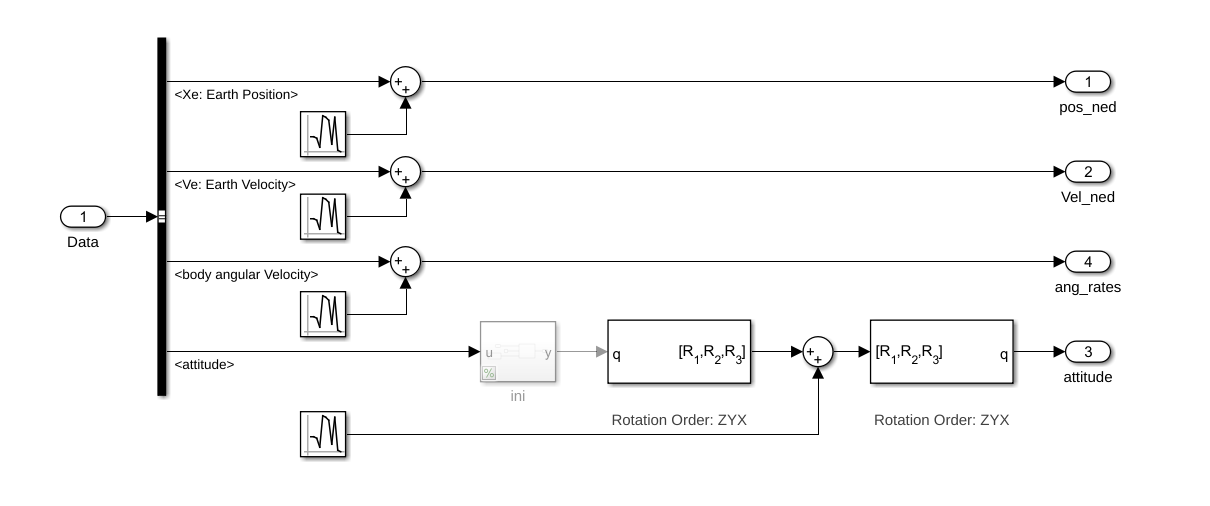
\includegraphics[width=0.95\linewidth]{Images/Current Status.png}
    \caption{Signal filter block}
    \label{fig:signal_filter_block}
\end{figure}

\subsection{Fixed-Wing Attitude Controller}
In this section, the attitude control system of the VTOL in the fixed-wing phase is presented in detail. The main structure is derived from \cite{px4controller}. Longitudinal and lateral dynamics are assumed to be uncoupled. The variables that have to be controlled are roll angle \( \phi \), pitch angle \( \theta \), and yaw rate \( \dot{\psi} \).

\subsubsection{Roll and Pitch Control}
The roll and pitch controllers follow a PID cascade loop structure (Figure \ref{fig:pid_cascade_loop}). The outer loop computes the error between the attitude setpoint \( \phi_{sp} \), \( \theta_{sp} \) and the estimated attitude \( \phi \), \( \theta \) respectively. This error, multiplied by the proportional gain \( P \), generates the Euler angle derivatives setpoint \( \dot{\phi}_{sp} \), \( \dot{\theta}_{sp} \), which is then converted into body rate setpoint \( p_{sp} \), \( q_{sp} \) with the matrix \( E \). The inner loop computes the rate error and utilizes proportional and integral controllers (PI) to produce the desired control surface deflections \( \delta_a \), \( \delta_e \) (aileron and elevator respectively).

The yaw controller generates its yaw rate setpoint using the turn coordination constraint to minimize lateral acceleration.

\begin{figure}[h]
    \centering
    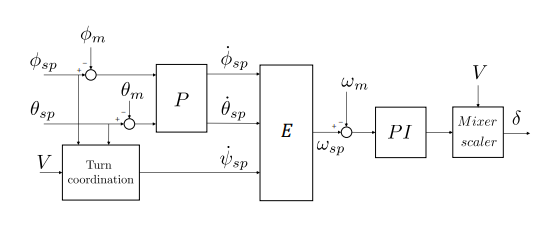
\includegraphics[width=1\linewidth]{Images/pid_cascade_loop.png}
    \caption{Fixed-wing Attitude Control Architecture: $\boldsymbol{\omega}$ is the body rates vector, $\boldsymbol{\delta}$ the control surfaces deflections vector ($\boldsymbol{\delta} = [\delta_a, \delta_e, \delta_r]$), and $V$ the airspeed.}
    \label{fig:pid_cascade_loop}
\end{figure}

\subsubsection{Yaw Rate Control: Turn Coordination}

During a turn maneuver (Figure \ref{fig:Forces during a turn}), the horizontal equilibrium yields:
\begin{equation}
    F_{\text{lift}} \sin \phi = mV \dot{\psi}
\end{equation}
where \( F_{\text{lift}} \) is the lift, \( V \) the aircraft speed, \( m \) the aircraft mass, and \( \dot{\psi} \) the yaw rate. The vertical component must balance gravity:
\begin{equation}
    F_{\text{lift}} \cos \phi = mg
\end{equation}
This leads to the yaw rate equation:
\begin{equation}
    \dot{\psi} = \frac{g}{V} \tan \phi \cos \theta
\end{equation}

A scaling factor \( K_{\text{scaler}} \) adjusts the control action based on airspeed \( V \), while saturation limits are applied to control surface deflections (Table \ref{tab:Maximum measured surfaces deflections.}).

\begin{figure}[h]
    \centering
    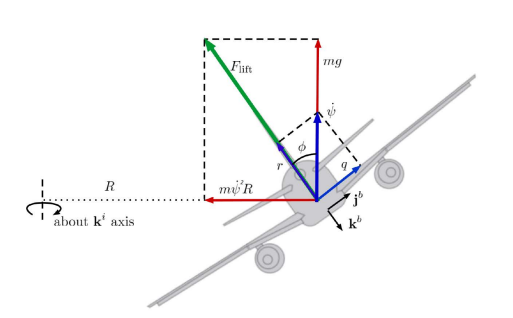
\includegraphics[width=0.9\linewidth]{Images/Forces during a turn, from [35].png}
    \caption{Forces during a turn}
    \label{fig:Forces during a turn}
\end{figure}

\begin{table}[h]
    \centering
    \begin{tabular}{ccc}
    \hline
        Rudder & Elevator & Aileron \\
    \hline
        \(50^\circ\) Left & \(60^\circ\) Down & \(35^\circ\) Down \\
        \(55^\circ\) Right & \(-50^\circ\) Up & \(-45^\circ\) Up \\
    \hline
    \end{tabular}
    \caption{Maximum measured surfaces deflections}
    \label{tab:Maximum measured surfaces deflections.}
\end{table}

\subsubsection{Total Energy Control System (TECS)}
In TECS (Total Energy Control System), managing both true airspeed and altitude simultaneously poses a challenge due to the coupled responses of the aircraft. Traditional Single-Input Single-Output (SISO) controllers handle each control variable separately, often leading to control coupling issues. TECS offers a solution by reframing the problem in terms of energies rather than original setpoints. By transforming initial setpoints into energy quantities, the control problem becomes decoupled. Thrust is then utilized to regulate the specific total energy of the aircraft, while pitch maintains a balance between potential and kinetic energy.

\subsubsection{Controller Algorithm}
The analysis presented here is derived from \cite{faleiro1999analysis}. The total energy of an aircraft is expressed as the sum of kinetic and potential energy, and its derivative leads to the total energy rate. Thrust setpoint is used for total energy control, while elevator is considered for energy distribution control. A simple control law, using proportional and integral control feedback, can be formulated. The control outputs are the normalized thrust and the pitch angle. Feedbacks of specific energy rate and energy balance rate are used to avoid the creation of unwanted zeros in the system transfer functions. The main structure of the algorithm is shown in Figure \ref{fig:TECS algorithm structure}.

\begin{figure}
    \centering
    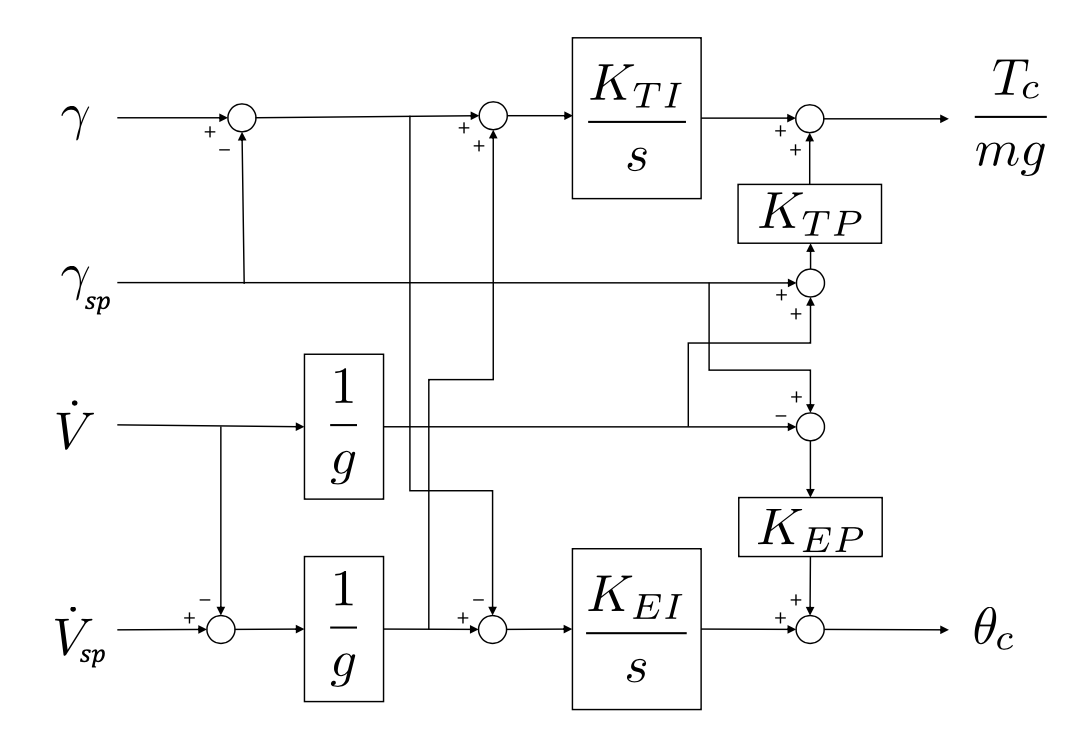
\includegraphics[width=0.9\linewidth]{Images/TECS algorithm structure..png}
    \caption{TECS algorithm structure.}
    \label{fig:TECS algorithm structure}
\end{figure}

\subsubsection{Controller Input and Output}
From a control perspective, the interest lies in altitude \( H_{sp} \) and speed \( V_{sp} \). The flight path angle \( \gamma_{sp} \) and the normalized longitudinal acceleration \( \frac{{\dot{V}_{sp}}}{{g}} \) are computed externally using a proportional controller on height and velocity error:
\begin{align}
    \dot{V}_{sp} &= K_v (V_{sp} - V), \\
    \dot{H}_{sp} &= K_H (H_{sp} - H), \\
    \gamma_{sp} &= \frac{{\dot{H}_{sp}}}{{V}}.
\end{align}
Speed and altitude errors are weighted equally to achieve decoupled control and efficient energy management during simultaneous flight path and speed maneuvers. Thus, the gains \( K_v \) and \( K_H \) should be equal \cite{faleiro1999analysis}.

These commands, \( \dot{V}_{sp} \) and \( \gamma_{sp} \), must be limited according to the aircraft performance to stay within a safe flight envelope.

For the input measurement \( \dot{V} \), it is suggested \cite{fari2017guidance} to take the acceleration measurement on the \( b_1 \) axis and subtract the contribution given by gravity:
\begin{equation}
    \dot{V} = a_x - g \sin \theta.
\end{equation}

The outputs of the TECS controller consist of a normalized thrust \( \frac{{T_c}}{{mg}} \) and a pitch angle \( \theta_c \). The latter is given as input into the attitude controller. Thus, the performance of TECS is directly affected by the performance of the pitch control loop.

The normalized thrust, after multiplication with the aircraft weight, is converted into throttle command \( \delta_t \) according to the following relations:
\begin{align}
    \Omega = \sqrt{\frac{{T_c}}{{K_T n_{\text{motors}}}}}
    \delta_t = \frac{{\Omega - q_{\text{fwd}}}}{{m_{\text{fwd}}}}
\end{align}
where \( \Omega \) is the angular speed of the motors. The coefficients \( K_T \), \( q_{\text{fwd}} \), and \( m_{\text{fwd}} \) have been computed in \cite{martello2021}.

\subsection{Optimization of the Throttle command generation block}
The original throttle command generation module operates under the assumption that the influence of incoming airflow can be neglected. However, this can lead to significant errors in estimating the thrust and torque generated by the propellers. To address this issue, a new Throttle Command Generation Module is developed, building upon the theoretical framework introduced in Section \ref{section:force elements} of Chapter \ref{ch:chapter1}. This new module utilizes equations (\ref{eq:thrust_1}) to (\ref{eq:outcome_airflow}) to predict the required motor angular velocity, thrusts, and torques based on this theory, thereby improving the accuracy of throttle commands.

Equation (\ref{eq:outcome_airflow}) requires knowledge of the motor's angular velocity and incoming airflow to calculate generated thrusts and torques. To ensure compatibility with real-world flight conditions, default throttle values are set for both fixed-wing and multi-copter modes. In fixed-wing mode, where the drone maintains a stable airspeed of $15 \text{ m/s}$, the throttle is set to $40\%$. Similarly, in multi-copter mode, where the drone is hovering, the assumed throttle value is set to $45\%$.

Additionally, due to the computational cost of the control system and the complexity of measuring incoming airflow for each propeller, a simplification in the calculation is necessary. Therefore, the incoming airflow is approximated by the body velocity of the drone itself. This simplification is justified by the negligible rotation speed of the drone compared to the cruise speed in fixed-wing mode and the climb/descent speed in multi-copter mode.

\begin{figure}
    \centering
    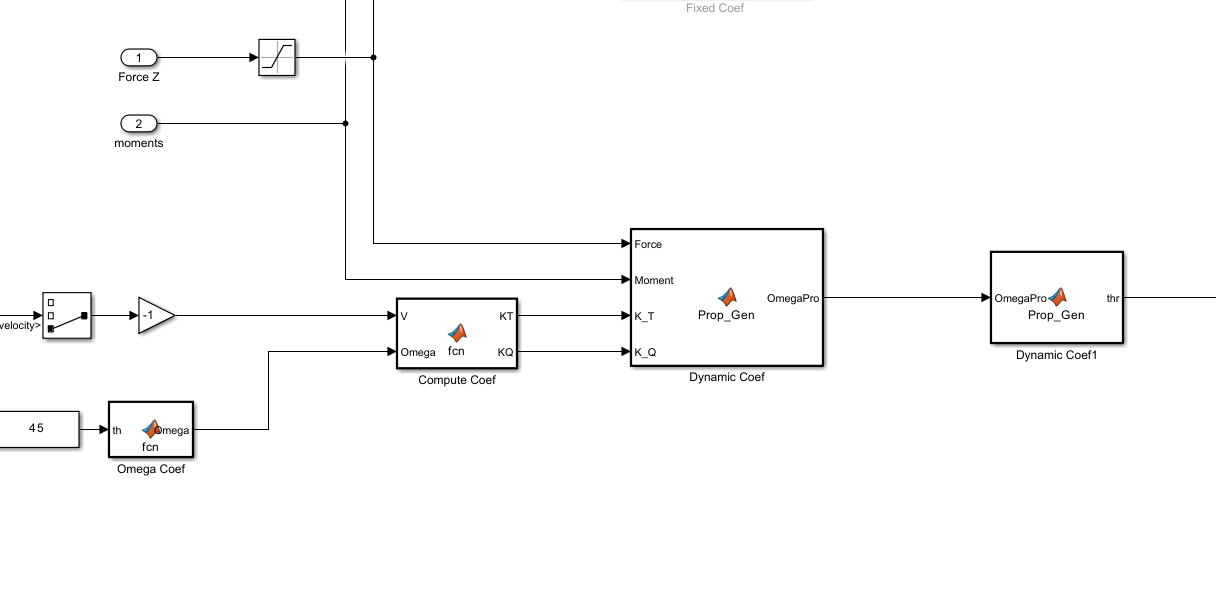
\includegraphics[width=0.9\linewidth]{Images/throttle command generation block.png}
    \caption{Throttle Command Generation Module.}
    \label{fig:Throttle Command Generation Module}
\end{figure}
